\section{Concurrent updates for Linux kernel}

\subsection{Case study:reverse mapping}
%Paragraph 1: Linux의 reverse mapping에 대한 자세한 설명 


\subsection{anon vma}

LDU. 
%Paragraph 1: anon vma에 ldu 적용한 방법에 대한 설명 


%Paragraph 2: anon vma에 적용하는데 문제점 설명 


PLDU. 
%Paragraph 1: anon vma에 적용


%Paragraph 2: Linux의 reverse mapping에 대한 자세한 설명 


\subsection{file mapping}

LDU. 
%Paragraph 1: Linux의 reverse mapping에 대한 자세한 설명 

%Paragraph 2: Linux의 reverse mapping에 대한 자세한 설명 



PLDU. 
%Paragraph 1: 

%Paragraph 2: Linux의 reverse mapping에 대한 자세한 설명 





%$$$$$$$$$$$$$$$$$$$$$$$$$$$$$$$$$$$$$$$$$$$$$$$$$$$$$$$$$$$$$$$$$$$$$$$$$$$$$$$$
%Reference Sentence 1
%$$$$$$$$$$$$$$$$$$$$$$$$$$$$$$$$$$$$$$$$$$$$$$$$$$$$$$$$$$$$$$$$$$$$$$$$$$$$$$$$

%$$$$$$$$$$$$$$$$$$$$$$$$$$$$$$$$$$$$$$$$$$$$$$$$$$$$$$$$$$$$$$$$$$$$$$$$$$$$$$$$
%Reference Sentence 2
%$$$$$$$$$$$$$$$$$$$$$$$$$$$$$$$$$$$$$$$$$$$$$$$$$$$$$$$$$$$$$$$$$$$$$$$$$$$$$$$$


%Figure : AIM7 실험 결과
%\begin{figure}[tb]
%  \begin{center}
%    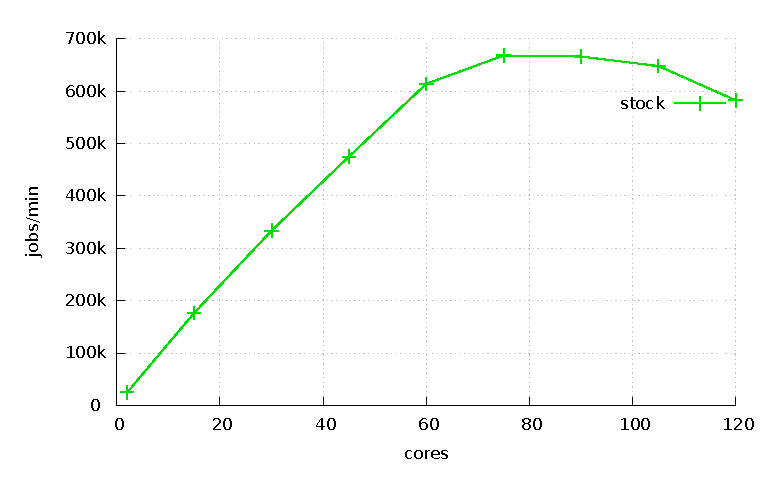
\includegraphics[scale=0.65]{graph/aim7_default.eps}
%  \end{center}
%  \caption{Scalability of AIM7 multiuser. This workload simultaneously create
%  many processes.
%  Up to 60 core, the stock Linux scale linearly, then they flattens out.}
%  \label{fig:aim7_default}
%\end{figure}
 
%In this section, we describe how to apply our concurrent update based on
%deferred update method to Linux.
%The Linux fork is associate with an anonymous page and a file page.
%When many processes are simultaneously created in Linux, 
%these two reverse mapping
%can become bottlenecks since their data structures are shared between
%processes.
%Figure~\ref{fig:aim7_default} shows the scalability problem in case
%of the fork-intensive workload that simultaneously creates many processes.
%Up to 60 core, the stock Linux scales linearly, then creating the reverse
%mapping becomes the bottleneck because their interval trees are protected by
%locks.
%Therefore, fork-intensive workload can pose a scalability bottleneck due to the
%update-heavy data
%structures~\cite{SilasBoydWickizerPth}~\cite{Andi2011adding}~\cite{Tim2013adding}.

%Figure mapped page에 대에 적용한  그림
%\begin{figure}[tb]
%%  \begin{center}
    %
    % \includegraphics[width=0.5\textwidth,height=0.5\textheight,keepaspectratio]{fig/deferu}
%  \end{center}
%  \caption{An example of applying the \deferu to file reverse mapping. }
%  \label{fig:deferu}
%\end{figure}


%Paragraph 6: DeferU 알고리즘 적용 - Mapped page - 리눅스 자료구조를 수정
%Figure~\ref{fig:deferu} gives an example of applying the \deferu to file
%reverse mapping and shows relationship between interval trees and lock-less
% lists.
%An interval tree contains two \code{virtual memory area}(\code{VMA}) nodes; 
%on the other hand, the lock-less list contains the right \code{VMA} as shown in
%Figure~\ref{fig:deferu}.
%It means that the right \code{VMA} has been deleted, and the synchronization
% has not been invoked. 

%In order to using the \deferu, the data structures involved in the
%head(\code{address\_space}) or the node(\code{vm\_area\_structure}) can be
% modified with \deferu's structure as shown in Figure~\ref{fig:deferu}. 
%In addition, programmer must replace \emph{physical update} with \emph{logical
%update} to eliminate the lock. 
%Before the corresponding readers need to be read, \deferu must call synchronize
%function to keep the consistency.
